\section{Exploring the Schedule Space}
\label{sec:exploring}

% \begin{itemize}
%   \item The scheduling language described in Section \ref{sec:schedule} allows
%   for numerous possible schedules for a given model. 
%   Finding a schedule with good performance is a non-trivial task.
%   \item We identify a reasonable template schedule for GPUs which encompasses
%   all strategies published in prior work.
%   \item Describe the template schedule.
%   \item Even within the variants of this template schedule, there is a significant 
%   amount of variation in performance. Show the histogram. 
%   \item Extensively exploring all possible parameter values for the template schedule 
%   is infeasible due to the large number of parameters.
%   Cite some numbers on how long it takes to explore the schedule space.
%   \item List the observations we make and the heuristic we design based on these.
% \end{itemize}
The set of schedules that can be constructed using the scheduling language described in 
Section \ref{sec:schedule} is unbounded.
%\TODO{kr: next few lines need more work}
% Even if one were to search for a good schedule offline, before deploying the model 
% on a specific hardware, additional tools are needed to help search for a 
% high-performance schedule. 
Additional tools are required to help search for a high-performance schedule.
Like with other schedule-guided ML compilers~\cite{TVM},
we expect schedule exploration will be performed offline (before a model deployment),
% But still, even for the most complex models, 
% one would like to spend at most a few minutes doing this search.
but spending more than a few minutes on this search is likely not acceptable.
We propose a set of heuristics to guide the search for a good schedule 
and meet this goal. These heuristics work by first defining a 
bounded search space and then pruning this search space further
based on the batch size and model characteristics.

\subsection{Bounding the search space}
We bound the space using a few meta-parameters that together define 
the primitives used to construct a schedule. We do so while making sure 
that the space (at-least) covers the known strategies published in prior work.
Specifically, we use the 9 parameters listed in Table \ref{tab:schedparams}.
We picked the specific values listed through experimentation.
%Note that even this template has a large number ($1728$) of schedules, and requires further pruning as we discuss later.
The first three numeric parameters assign a configurable number of rows to each 
thread block, to each thread, and determine how trees are distributed across a
specified number of threads. These parameters together define the loop schedule 
primitives to use (including the arguments to pass) from Table~\ref{Tab:LoopModifiers} 
and the parallelization strategy. The next four parameters determine the caching strategy, 
unroll factor{\footnote{We choose to always unroll trees completely, while its possible 
to partially unroll loops we did not observe any performance benefits from doing so.}} 
and how many trees to traverse simultaneously within
a single thread (the remaining primitives from Table~\ref{Tab:Optimizations}).  
The last two parameters determine reduction optimizations (Table~\ref{Tab:ReductionOpts}) 
and the layout{\footnote{This does not have a schedule primitive. We always explore all three layout options.}} to use.
%Table \ref{tab:schedparams} lists the parameter values we tried. 
% \begin{itemize}
%   \item \textbf{Number of rows per thread block (Integer):} The number of rows that are processed by each thread block.
%   \item \textbf{Number of rows per thread (Integer):} The number of rows processed by each thread.
%   \item \textbf{Number of tree threads (Integer):} The number of threads across which the trees are distributed.
%   \item \textbf{Cache rows (Boolean):} Whether the input rows are cached in shared memory.
%   \item \textbf{Cache trees (Boolean):} Whether the trees are cached in shared memory.
%   \item \textbf{Unroll walks (Boolean):} Whether the tree walks are unrolled.
%   \item \textbf{Tree walk interleave factor:} The number of tree walks that are interleaved.
%   \item \textbf{Shared memory reduction:} Whether the reduction across tree threads is done in shared memory.
% \end{itemize}

\begin{table}[htb]
  \footnotesize
  \centering
  % \resizebox{\linewidth}{!}{
  \begin{tabularx}{\linewidth}{c | c }
    \toprule
    \textbf{Parameter} & \textbf{Values} \\
    \midrule
    \textbf{Rows per thread block} & $\{8, 32, 64\}$ \\
    \textbf{Rows per thread} & $\{1, 2, 4\}$ \\
    \textbf{Number of tree threads} & $\{2, 10, 20, 50\}$ \\
    \textbf{Cache rows} & $\{True, False\}$ \\
    \textbf{Cache trees} & $\{True, False\}$ \\
    \textbf{Unroll walks} & $\{True, False\}$ \\
    \textbf{Tree walk interleave factor} & $\{1, 2, 4\}$ \\
    \textbf{Shared memory reduction} & $\{True, False\}$ \\
    \textbf{Representation} & $\{array, sparse, reorg\}$ \\
    \bottomrule
  \end{tabularx}
  % }
  \vskip 5pt
  \caption{\label{tab:schedparams} List of parameter values we explored for the template GPU schedule.}
\end{table}

%While the template schedule simplifies optimization of generated inference code,
It is important to note that the \Treebeard{} compiler itself does not place any 
restrictions on the schedule. The user is free to specify any schedule they wish.
The compiler pass that implements the template schedule is also implemented as a 
module outside the core \Treebeard{} compiler. 
% Users are also free to implement 
% other auto-schedulers that generate schedules different from the template schedule.

\begin{figure}[htb]
  \centering
  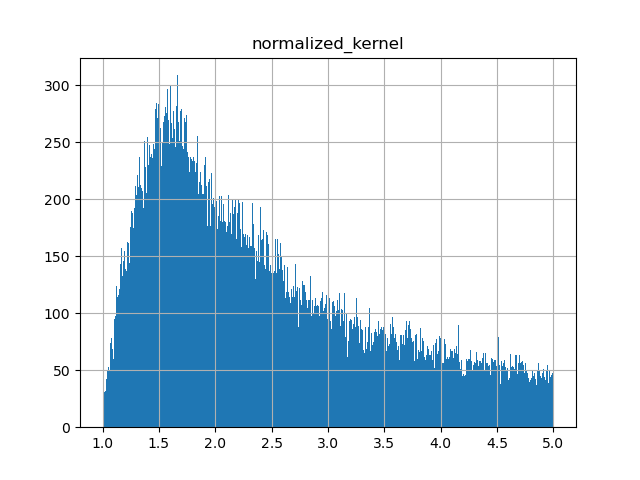
\includegraphics[width=0.85\linewidth]{figures/normalized_kernel_histogram_lt5.png}
  \caption{Distribution of normalized execution times for real-world benchmark models
  with different combinations of parameter values shown in Table \ref{tab:schedparams}}. 
  \label{Fig:ExecTimeDistribution}
\end{figure}

We evaluated all the schedules in this space on several real world models and observed that 
there is huge variation in performance with different parameter values. 
Figure \ref{Fig:ExecTimeDistribution} shows the distribution of normalized execution times
for our real-world benchmark models with different parameter values (inference
times normalized w.r.t fastest time for that model).
As can be seen, very few schedules perform close to the best while a vast majority perform poorly.

Exhaustive exploration over this bounded space ($5184$ schedules) is still very expensive, taking
between $30-300$ minutes to explore the entire space for a given model. 
%Exploring the space for every model is infeasible.
%\TODO{comment on online vs offline exploration? Set a goal for the heuristic?}

\subsection{Pruning the search space}
%Exploring the schedule space extensively even for a reasonable set of parameter values is very expensive.
 
%Performing this extensive search for every model being compiled is infeasible in practise. 
A careful analysis of the search space reveals that certain schedules are not likely to 
perform well as they either do not exploit the parallelism available in the model or do not take advantage of the hardware features.
We use a combination of 3 strategies to further prune the search space.
Algorithm \ref{alg:heuristic} presents our final heuristic to find a good schedule.
%need a better mechanism to guide the search for a good schedule.

\subsubsection*{Insufficient parallelism}
 Some configurations do not expose sufficient parallelism, we prune these out.
  For example when the batch size is small, it does not make sense to have many rows
  per thread block or to partition the trees across a few threads. 
  We therefore limit the combinations used based on batch size (see lines 3---8).
\subsubsection*{Utilizing shared memory}
  Shared memory is a critical resource on GPUs and it helps to only bring objects that would be reused into it. 
  We observe that tree nodes have limited reuse and the one time cost of loading trees is not sufficiently amortized when the whole tree is not accessed during inference. 
  On the other hand caching rows 
  %when possible (i.e., when the number of features is small enough to fit in shared memory)
  almost always improves performance. Further when the inputs have many features, it may not be possible to cache all rows.
  In this scenario it helps to retain a few rows in memory, and pick schedules similar to the small batch size case (lines 15,3---5).

  %trees across more threads even at larger batch sizes. This is because processing fewer rows at a time 
  %allows us to keep them in shared memory.
  % We empirically find that the threshold for when 
  % we should start partitioning the trees across more threads is when the number of features
  % is greater than 100. 
  \subsubsection*{Orthogonal parameters} We find that some parameters like reduction type are orthogonal to the rest. 
  We therefore break the exploration into two phases, first we pick the best schedules without reduction
  optimizations and then evaluate reduction options on the best schedules.
  %We find that when a model prefers schedules with shared reduction, the same schedules 
  %without shared reduction are among the best performing schedules without shared reduction.
  % We therefore are able to separate the evaluation of shared reduction by collecting the 
  % best schedules without shared reduction and only evaluating shared reduction on them. 
  Evaluating the top 3 schedules for reduction is sufficient in practice.  

\begin{comment}
\Treebeard{} uses these observations to narrow down the set of schedules to explore. 
The pseudo-code for the heuristic is shown in Algorithm \ref{alg:heuristic}.
The algorithm first computes a subset of thread block configurations in the function 
\op{TBConfigs}. A set of schedules based on these thread block configurations 
is then computed (\op{schedules}). 
\end{comment}

\noindent
\Treebeard{} performs an exhaustive search over the pruned schedules to find the best schedule.
The model is compiled with each of these schedules and evaluated on a few input batches. 
%The three best performing schedules 
%are collected and shared reduction is enabled on them and the resulting schedules evaluated.
The best schedule among all the evaluated schedules is selected as the schedule to use.
We report that this heuristic is able to find schedules that are close to the best schedules
while improving the search time by two orders of magnitude (see Section \ref{sec:results}).

\begin{algorithm}
  \caption{Heuristic to find a good schedule}
  \label{alg:heuristic}
  \footnotesize{
  \begin{algorithmic}[1]
  \Procedure{TBConfigs}{$N_{batch}$, $N_f$}
    \State $T_{batch} \gets 2048,\; T_f \gets 128$
    \If {$N_{batch} \leq T_{batch}$ \textbf{or} $N_{f} > T_{f}$}
      \State $rowsPerBlock \gets \{8, 32\}$
      \State $treeThreads \gets \{20, 50\}$
    \Else
      \State $rowsPerBlock \gets \{32, 64\}$
      \State $treeThreads \gets \{2, 10\}$
    \EndIf
    \State \Return $rowsPerBlock, treeThreads$
  \EndProcedure
  \\
  \State $bestSchedules \gets shMemSchedules \gets \emptyset$
  \State $rowsPerTB, treeThds \gets TBConfigs(N_{batch}, N_f)$
  \State $cacheRows \gets \text{True},\; cacheTrees \gets \text{False}$
  \State $interleave \gets \{1, 2, 4\}$
  % \State $reps \gets \{array, sparse, reorg\}$
  \State $schedules \gets (rowsPerTB, treeThds, cacheRows,$ \\
                          \hspace{2cm}$cacheTrees, interleave)$
                          %\hspace{2cm}$$
  \For{$(sched, rep) \in schedules \times \{array, sparse, reorg\}$}
    \State $time \gets EvaluateSchedule(sched, rep)$
    \State $bestSchedules.insert(time, sched, rep)$
  \EndFor
  \State 
  \For{$sched, rep \in Top3(bestSchedules)$}
    \State $EnableSharedReduction(sched)$
    \State $time \gets EvaluateSchedule(sched, rep)$
    \State $shMemSchedules.insert(time, sched, rep)$
  \EndFor
  \State \Return $min(shMemSchedules \cup bestSchedules)$
  \end{algorithmic} 
  }
\end{algorithm}